\documentclass{standalone}
%<--------------------------------------------------------------------------->%
%%% Color %%%
\usepackage[dvipsnames]{xcolor} % \textcolor{red}{}
\definecolor{rot}{RGB}{229,0,0}
\definecolor{bla}{RGB}{0,98,144}
\definecolor{gel}{RGB}{255,195,0}
%<--------------------------------------------------------------------------->%

%<--------------------------------------------------------------------------->%
%%% TikZ %%%
\usepackage{tikz}
\usetikzlibrary{calc}
% \usetikzlibrary{fit}
% \usetikzlibrary{angles,quotes}
% \usetikzlibrary{intersections,topaths}
% \usetikzlibrary{decorations.markings}
%<--------------------------------------------------------------------------->%
%%% TikZ: Mark Angles %%%
\newcommand{\MarkRightAngle}[5][]{%
\draw[#1] let \p1=($(#3)-(#4)$),\n1={1/veclen(\x1,\y1)},\p2=($(#4)-(#5)$),\n2={1/veclen(\x2,\y2)}in%
($(#4)!#2!(#5)$) -- ++(\x1*\n1*#2,\y1*\n1*#2) -- ++(\x2*\n2*#2,\y2*\n2*#2);}
\newcommand{\MarkAngle}[5]["$\theta$",->,draw=blue!80,fill=blue!20]{\pic[#1,angle radius=#2] {angle = #3--#4--#5};}
%<--------------------------------------------------------------------------->%

\begin{document}

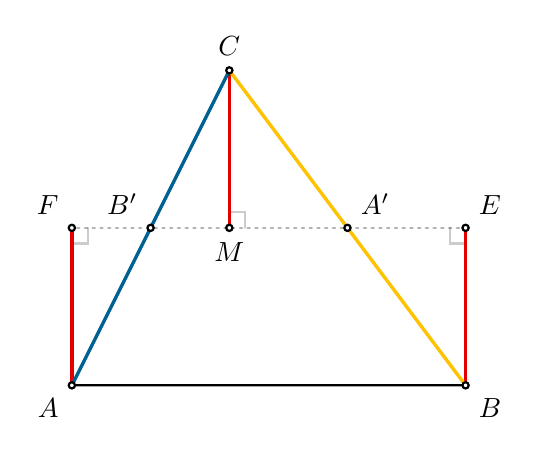
\begin{tikzpicture}[thick,line cap=round]
	\tikzstyle{jiao}=[solid,circle,draw,fill=white,inner sep=.8pt];
	\tikzstyle{rightangle}=[opacity=0.2];
\newcommand{\rightanglesize}{0.2cm}
\tikzstyle{normalangle}=[fill=bla,opacity=0.2];
\newcommand{\anglesize}{0.5cm}
\tikzstyle{help}=[dotted,opacity=0.2];
%<--------------------------------------------------------------------------->%

	\newcommand{\height}{4cm}
	\coordinate (A)  at (0,0);
	\coordinate (B)  at (5,0);
	\coordinate (C)  at (2,\height);
	\coordinate (a)  at ($(A)+(0,\height/2)$);
	\coordinate (b)  at ($(B)+(0,\height/2)$);
	\coordinate (AC) at ($(A)!0.5!(C)$);
	\coordinate (BC) at ($(B)!0.5!(C)$);
	\coordinate (M)  at ($(C)+(0,-\height/2)$);
	\draw (A) -- (B) -- (C) --cycle;
	\draw[opacity=0.3,dotted] (A) |- (AC) -- (BC) -| (B);
	\draw[opacity=0.3,dotted] (M) -- (C);
	%% Mark angles
	\MarkRightAngle[rightangle]{\rightanglesize}{BC}{M}{C};
	\MarkRightAngle[rightangle]{\rightanglesize}{BC}{b}{B};
	\MarkRightAngle[rightangle]{\rightanglesize}{A}{a}{AC};
	%% Mark Lines
	\draw[very thick,rot] (A) -- (a);
	\draw[very thick,rot] (C) -- (M);
	\draw[very thick,rot] (b) -- (B);
	\draw[very thick,bla] (AC) -- (C);
	\draw[very thick,bla] (AC) -- (A);
	\draw[very thick,gel] (BC) -- (B);
	\draw[very thick,gel] (BC) -- (C);
	%% Final
	\node[jiao,label=below left:{$A$}] at (A) {};
	\node[jiao,label=below right:{$B$}] at (B) {};
	\node[jiao,label=above:{$C$}] at (C) {};
	\node[jiao,label=below:{$M$}] at (M) {};
	\node[jiao,label=above right:{$E$}] at (b) {};
	\node[jiao,label=above left:{$F$}] at (a) {};
	\node[jiao,label=above left:{$B'$}] at (AC) {};
	\node[jiao,label=above right:{$A'$}] at (BC) {};
\end{tikzpicture}

\end{document}
